
\section{Verification}\label{sec:verif}
\optsection{Verification}

\bigskip
\begin{quote}  Two types of errors may be distinguished: modeling errors and numerical errors.  Modeling errors arise from not solving the right equations.  Numerical errors result from not solving the equations right.  The assessment of modeling errors is \emph{validation}, whereas the assessment of numerical errors is called \emph{verification} \dots  Validation makes sense only after verification, otherwise agreement between measured and computed results may well be fortuitous.
\end{quote}\index{validation versus verification}
\hfill P.~Wesseling, (2001)  \emph{Principles of Computational Fluid Dynamics}, pp.~560--561 \cite{Wesseling}
\bigskip

\subsection{Ideas}  Verification\index{PISM!verification of} is the essentially mathematical task of checking that the predictions of the numerical code are close to the predictions of a continuum model, the one which the numerical code claims to approximate.  It is a crucial task for a code as complicated as PISM. In verification there is no comparison between model output and observations of nature.  Instead, one compares exact solutions of the continuum model, in circumstance in which they are available, to their numerical approximations.

Reference \cite{Roache} gives a broad discussion of verification and validation in computational fluid dynamics. See \cite{BLKCB} and \cite{BBL} for discussion of verification issues for the isothermal and thermomechanically coupled shallow ice approximation (SIA), respectively, and for exact solutions to these models, and \cite{BBssasliding,SchoofStream} for verification using an exact solution to the SSA equations for ice streams.  

In PISM there is a separate executable \texttt{pismv}, which is used
for SIA-related verification, and there are additional scripts for SSA-related
verification.  The source codes which are verified by \texttt{pismv} are,
however, exactly the same source files, as are run by the
non-verification executables \texttt{pismr}, \texttt{pisms}, etc.  In
technical terms, \texttt{pismv} runs a derived class of the PISM base class.

\begin{table}[ht]
\centering
\caption{Exact solutions for verification.}\label{tab:tests}
\small
\begin{tabular}{p{0.1\linewidth}p{0.4\linewidth}p{0.25\linewidth}p{0.15\linewidth}}\toprule
\textbf{Test} & \textbf{Continuum model tested} & \textbf{Comments} & \textbf{Reference} \\ \midrule
A & isothermal SIA, steady,  flat bed, constant accumulation &  & \cite{BLKCB} \\
B & isothermal SIA, flat bed, zero accum & similarity soln & \cite{BLKCB,Halfar83} \\
C & isothermal SIA, flat bed, growing accum & similarity soln & \cite{BLKCB} \\
D & isothermal SIA, flat bed, oscillating accum & compensatory accum & \cite{BLKCB} \\
E & isothermal SIA; as A  but with sliding in a sector &  compensatory accum & \cite{BLKCB} \\
F & thermomechanically coupled SIA (mass and energy cons.), steady, flat bed &  compensatory accum and comp~heating& \cite{BB,BBL} \\
G & thermomechanically coupled SIA; as F  but with oscillating accumulation  & ditto & \cite{BB,BBL} \\
H & bed deformation coupled with isothermal SIA & joined similarity & \cite{BLKfastearth} \\
I & stream velocity computation using SSA (plastic till) &  & \cite{SchoofStream,BBssasliding} \\
J & shelf velocity computation using SSA  &  & [IN PREP] \\
K & pure conduction in ice and bedrock & & \cite{BuelerTestK} \\
L & isothermal SIA, steady, non-flat bed & numerical ODE soln & [IN PREP] \\
\bottomrule
\normalsize
\end{tabular}
\end{table}

\begin{table}[ht]
\centering
\caption{Canonical PISM \index{executables!\texttt{pismv}!options to run verification tests}\index{verification tests} verification runs using the exact solutions listed in table \ref{tab:tests}.}\label{tab:tests-exec}
\small
\begin{tabular}{@{}llll}\toprule
\textbf{Test} & \textbf{Example invocation}  \\ \midrule
A & \texttt{pismv -test A -Mx 61 -My 61 -Mz 11 -y 25000} \\
B & \texttt{pismv -test B -Mx 61 -My 61 -Mz 11 -ys 422.45 -y 25000}  \\
C & \texttt{pismv -test C -Mx 61 -My 61 -Mz 11 -y 15208.0}  \\
D & \texttt{pismv -test D -Mx 61 -My 61 -Mz 11 -y 25000}  \\
E & \texttt{pismv -test E -Mx 61 -My 61 -Mz 11 -y 25000}  \\
F & \texttt{pismv -test F -Mx 61 -My 61 -Mz 61 -y 25000}  \\
G & \texttt{pismv -test G -Mx 61 -My 61 -Mz 61 -y 25000}  \\
H & \texttt{pismv -test H -Mx 61 -My 61 -Mz 11 -y 40034 -bed_def_iso} \\
I & FIXME: use .py \texttt{ssa_testi -ssa_method fd -Mx 5 -My 500 -ssa_rtol 1e-6 -ksp_rtol 1e-11 } \\
J & FIXME: use .py \texttt{ssa_testj -ssa_method fd -Mx 60 -My 60 -Mz 11 -ksp_rtol 1e-12} \\
K & \texttt{pismv -test K -Mx 6 -My 6 -Mz 401 -Mbz 101 -y 130000} \\
L & \texttt{pismv -test L -Mx 61 -My 61 -Mz 31 -y 25000} \\
\bottomrule
\normalsize
\end{tabular}
\end{table}

\begin{table}[ht]
  \centering
  \caption{pismv command-line options}
  \begin{tabular}{lp{0.7\linewidth}}
    \toprule
    \textbf{Option} & \textbf{Description} \\
    \midrule
    \intextoption{test} & Choose which verification test to run by giving its
    single character name; see table \ref{tab:tests}.\\
    \intextoption{no_report} & Do not report errors at the end of a verification run.\\
    \intextoption{eo} & Only evaluate the exact solution (don't do numerical
    approximation at all).
   \\\bottomrule
  \end{tabular}
 \label{tab:pismv-options}
\end{table}

Table \ref{tab:tests} summarizes the many exact solutions currently available in PISM.  Most of these exact solutions are solutions of \emph{free boundary problems} for partial differential equations; only Tests A, E, J, K are fixed boundary value problems.  Table \ref{tab:tests-exec} shows how to run each of them on a coarse grids.  Table \ref{tab:pismv-options} gives the special verification-related options of the \texttt{pismv} executable.

Numerical errors are not, however, the dominant reasons why ice sheet models give imperfect results.  The largest sources of errors include those from using the wrong (e.g.~over-simplified or incorrectly-parameterized) continuum model, and from observational or pre-processing errors present in input data.  Our focus here on numerical errors has a model-maintenance goal.  It is \emph{easier} to maintain code by quantitatively confirming that it produces small errors in cases where those can be measured, rather than ``eyeballing'' results to see that they are ``right'' according to human judgment.

\subsection{Refinement}  The goal of verification is not generally to see that the error is zero at any particular resolution, or even to show that the error is small in a predetermined absolute sense.  Rather the goals are
\begin{itemize}
\item to see that the error \emph{is} decreasing,
\item to measure the rate at which it decreases, and
\item to develop a sense of the magnitude of numerical error which occurs in a realistic ice sheet model run.
\end{itemize}
Knowing the error decay rate may give a prediction of how fine a grid is necessary to achieve a desired smallness for the numerical error.

Therefore one must ``go down'' a grid refinement ``path'' and measure numerical error for each grid \cite{Roache}.  The refinement path is defined\index{refinement path!definition} by a sequence of spatial grid cell sizes which decrease toward the refinement limit of zero size \cite{MortonMayers}.  In PISM the timestep $\Delta t$ is determined adaptively by a stability criterion (see subsection \ref{subsect:adapt}).  In PISM one specifies the number of grid points, thus the grid cell sizes because the overall dimensions of the computational box are normally fixed; see subsection \ref{subsect:coords}.  By ``measuring the error for each grid'' we mean computing a norm (or norms) of the difference between the numerical solution and the exact solution.

For example, in tests of the thermomechanically-coupled SIA model one refines in three dimensions, and these runs produced figures 13, 14, and 15 of \cite{BBL}:\index{refinement path!example}
\begin{quote}\small
\begin{verbatim}
pismv -test G -max_dt 10.0 -y 25000 -Mx 61 -My 61 -Mz 61 -z_spacing equal
pismv -test G -max_dt 10.0 -y 25000 -Mx 91 -My 91 -Mz 91 -z_spacing equal
pismv -test G -max_dt 10.0 -y 25000 -Mx 121 -My 121 -Mz 121 -z_spacing equal
pismv -test G -max_dt 10.0 -y 25000 -Mx 181 -My 181 -Mz 181 -z_spacing equal
pismv -test G -max_dt 10.0 -y 25000 -Mx 241 -My 241 -Mz 241 -z_spacing equal
pismv -test G -max_dt 10.0 -y 25000 -Mx 361 -My 361 -Mz 361 -z_spacing equal
\end{verbatim}
\normalsize\end{quote}
The last two runs require a supercomputer!  In fact the $361\times 361\times 361$ run involves more than $100$ million unknowns, updated at each of millions of time steps. Appropriate use of parallelism (\texttt{mpiexec -n NN pismv}) and of the \texttt{-skip} modification to adaptive timestepping accelerates such fine-grid runs; see section \ref{sec:practical-usage}.


\subsection{Sample verification results}  Figures \ref{fig:thickerrsB} through
\ref{fig:velerrsI} show a sampling of the results of verifying PISM using the
tests described above.\index{PISM!verification results and reporting}  These
figures were produced automatically using Python scripts
\texttt{test/vfnow.py} \index{executables!python scripts!\texttt{vfnow.py}} and \texttt{test/vnreport.py}.\index{executables!python scripts!\texttt{vnreport.py}}  See subsection \ref{subsect:scripts}.

These figures \emph{do not} show outstanding rates of convergence, relative to textbook partial differential equation examples.  For the errors in tests B and G, see the discussion of free margin shape in \cite{BLKCB}.  For the errors in test I, note the low degree of smoothness of the continuum solution at the free boundary \cite{SchoofStream}.  

\begin{figure}[ht]
\centering
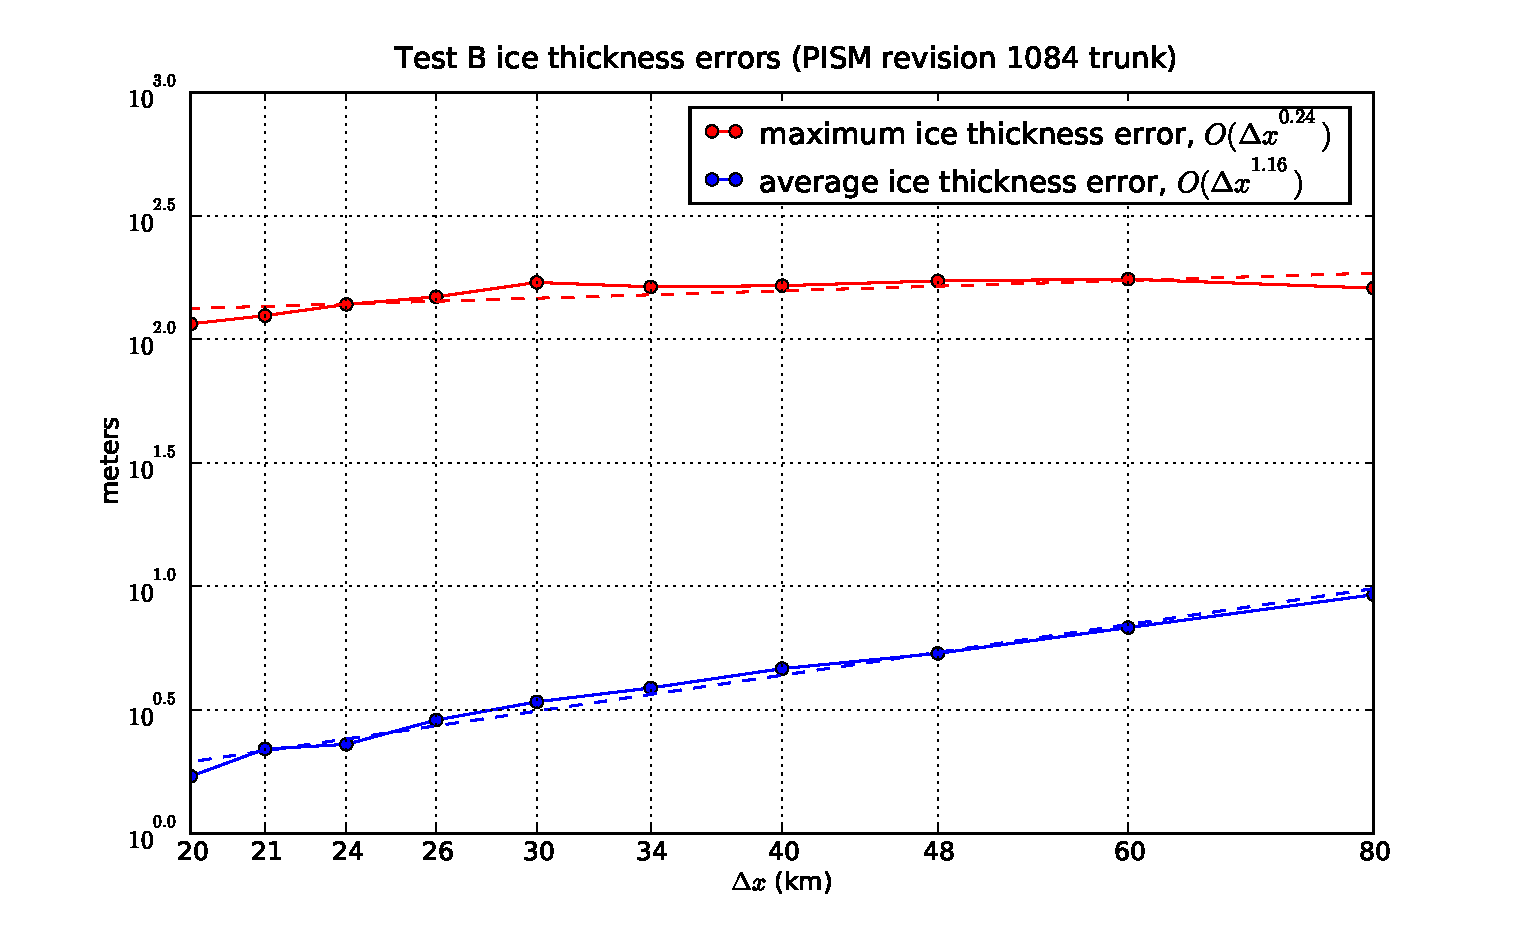
\includegraphics[width=4.8in,keepaspectratio=true]{test-B-thickness}
\caption{Numerical thickness errors in test B. See \cite{BLKCB} for discussion.}
\label{fig:thickerrsB}
\end{figure}

\begin{figure}[ht]
\centering
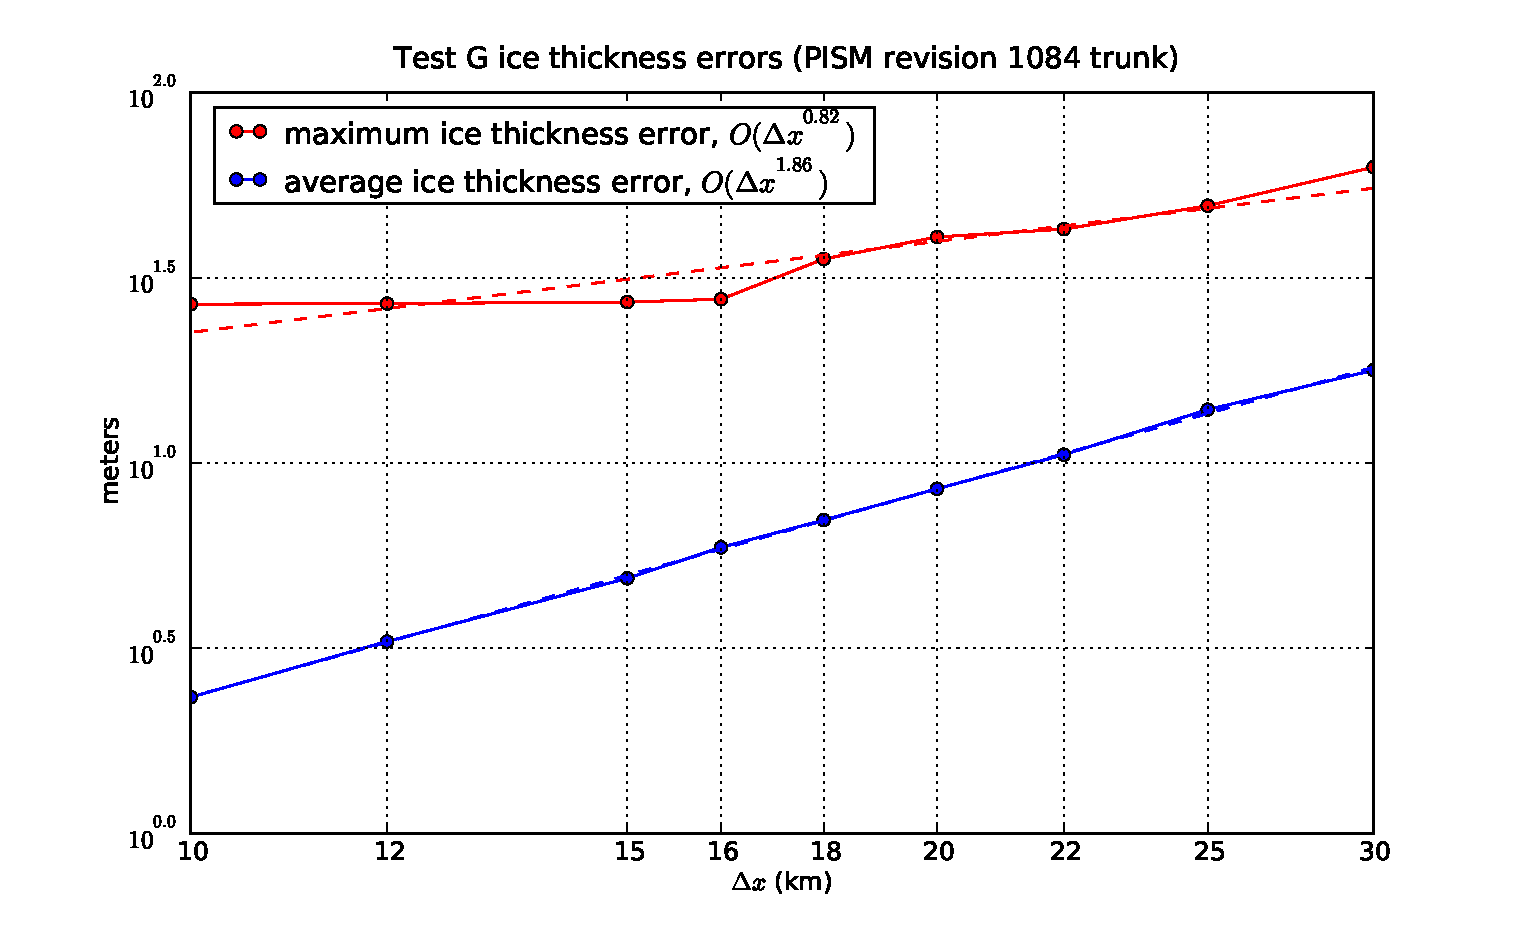
\includegraphics[width=5.0in,keepaspectratio=true]{test-G-thickness}
\caption{Numerical thickness errors in test G.  See \cite{BBL} and \cite{BLKCB}.}
\label{fig:thickerrsG}
\end{figure}

\begin{figure}[ht]
\centering
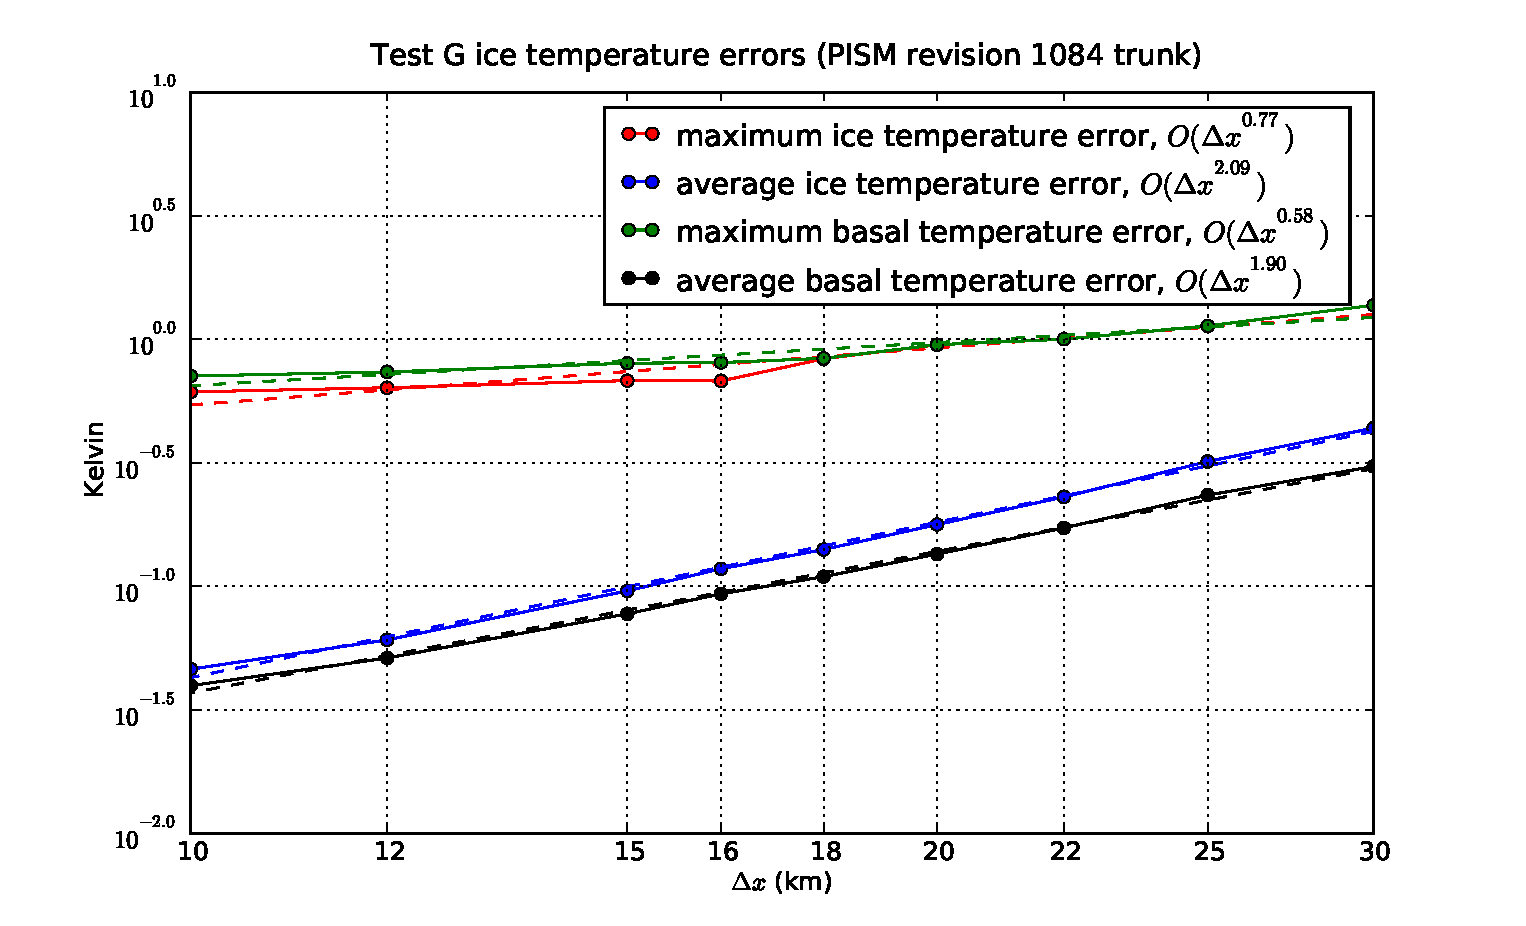
\includegraphics[width=5.0in,keepaspectratio=true]{test-G-temp}
\caption{Numerical temperature errors in test G. See \cite{BBL}.}
\label{fig:temperrsG}
\end{figure}

\begin{figure}[ht]
\centering
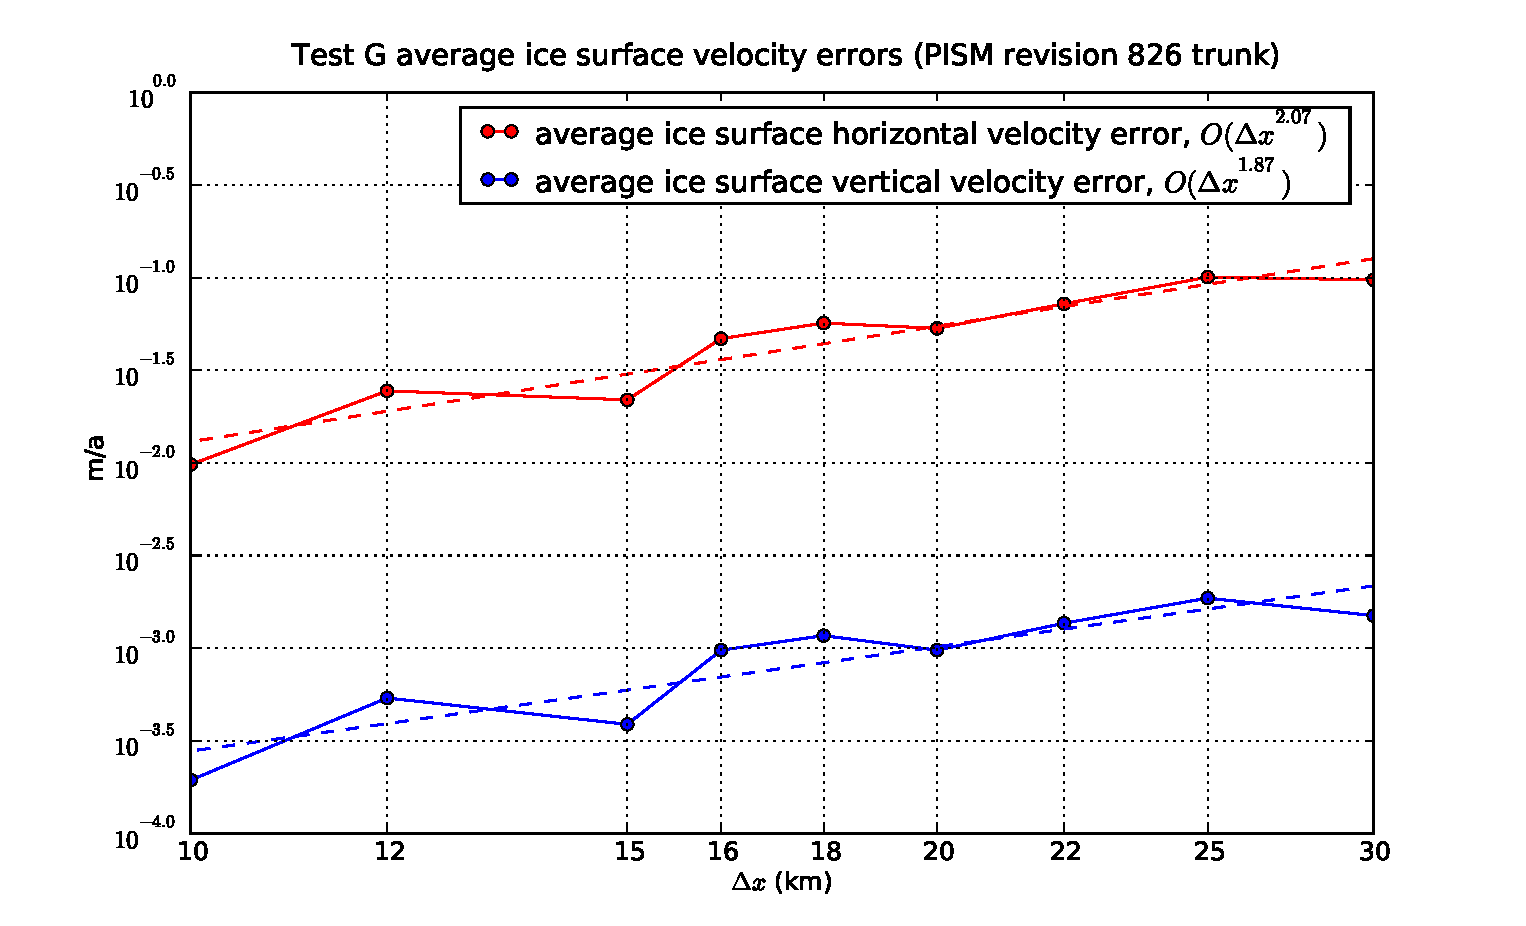
\includegraphics[width=5.0in,keepaspectratio=true]{test-G-surfvels}
\caption{Numerical errors in computed surface velocities in test G.}
\label{fig:surfvelerrsG}
\end{figure}

\begin{figure}[ht]
\centering
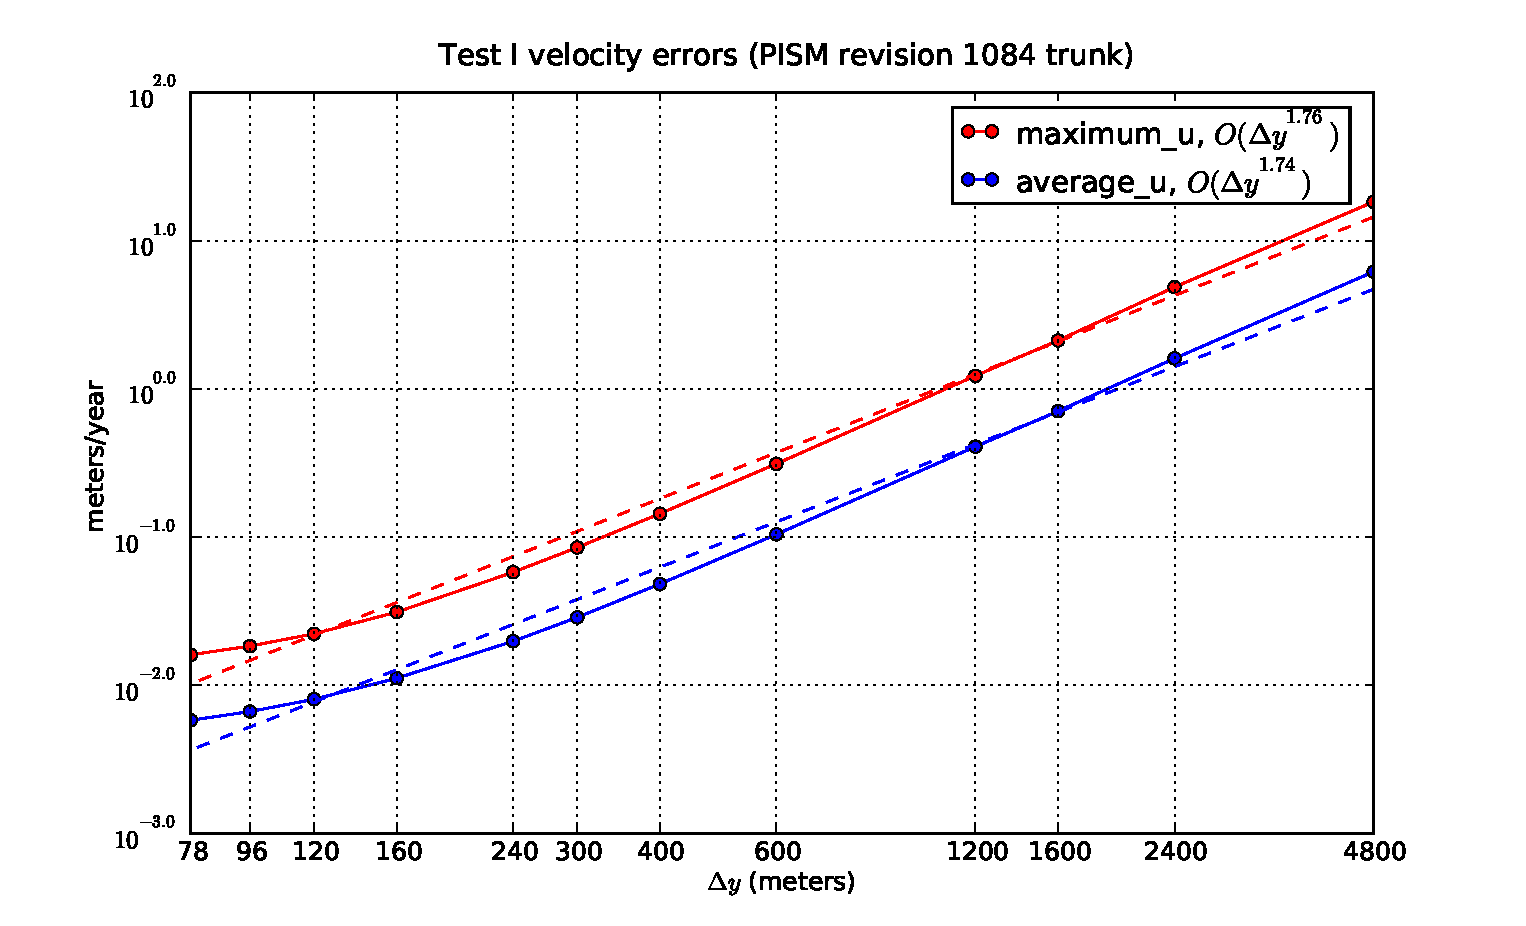
\includegraphics[width=5.0in,keepaspectratio=true]{test-I-errors}
\caption{FIXME:  verification scripts need updating to reproduce this.  Numerical errors in horizontal velocities in test I, an ice stream. \t{maximum_u} and \t{average_u} are errors in scalar velocity (because of symmetries in test I).  See \cite{SchoofStream,BBssasliding}.}
\label{fig:velerrsI}
\end{figure}



%%% Local Variables: 
%%% mode: latex
%%% TeX-master: "manual"
%%% End: 
